\documentclass[times, utf8, seminar, numeric]{fer}
\usepackage[utf8]{inputenc}
\usepackage[T1]{fontenc}
\usepackage{currvita}
\usepackage{graphicx}
\usepackage{epstopdf}
\usepackage{listings}
\usepackage{textcomp}
\usepackage{booktabs}
\usepackage{algorithmic}
\usepackage{algorithm}


% definicija jezika koji nema nista, pa se nista ne naglasava
% koristi se za troadresni kod, ispise tokena i slicno
\lstdefinelanguage{blank}{
	sensitive=false, 
	morecomment=[l]{;},
}

% neke boje koje koristimo u formatiranju ispisa
\usepackage{color}
\definecolor{mygreen}{rgb}{0,0.6,0}
\definecolor{mylightgray}{rgb}{0.95,0.95,0.95}

% definicija formatiranja ispisa, ponesto promjenjena u odnosu na pretpostavljenu
\lstset{ %
  backgroundcolor=\color{mylightgray},   % choose the background color; you must add \usepackage{color} or \usepackage{xcolor}
  basicstyle=\footnotesize\ttfamily,        % the size of the fonts that are used for the code
  breakatwhitespace=false,         % sets if automatic breaks should only happen at whitespace
  breaklines=true,                 % sets automatic line breaking
  captionpos=b,                    % sets the caption-position to bottom
  commentstyle=\color{mygreen},    % comment style
  deletekeywords={...},            % if you want to delete keywords from the given language
  escapeinside={\%*}{*)},          % if you want to add LaTeX within your code
  extendedchars=true,              % lets you use non-ASCII characters; for 8-bits encodings only, does not work with UTF-8
  frame=none,                    % adds a frame around the code
  keepspaces=true,                 % keeps spaces in text, useful for keeping indentation of code (possibly needs columns=flexible)
  keywordstyle=\color{blue},       % keyword style
  language=c,           	       % the language of the code
  morekeywords={*,...},            % if you want to add more keywords to the set
  numbers=none,                    % where to put the line-numbers; possible values are (none, left, right)
  numbersep=5pt,                   % how far the line-numbers are from the code
  numberstyle=\tiny\color{gray}, % the style that is used for the line-numbers
  rulecolor=\color{black},         % if not set, the frame-color may be changed on line-breaks within not-black text (e.g. comments (green here))
  showspaces=false,                % show spaces everywhere adding particular underscores; it overrides 'showstringspaces'
  showstringspaces=false,          % underline spaces within strings only
  showtabs=false,                  % show tabs within strings adding particular underscores
  stepnumber=2,                    % the step between two line-numbers. If it's 1, each line will be numbered
  stringstyle=\color{red},     % string literal style
  tabsize=2,                       % sets default tabsize to 2 spaces
  title=\lstname                   % show the filename of files included with \lstinputlisting; also try caption instead of title
}

\title{Detekcija lica u grupnim scenama}

\author{T. Antunović, S. Čolaković, E. Smoljan, F. Stamenković, I. Weber}

\voditelj{Marijo Maračić}


\begin{document}

\maketitle

\tableofcontents

\chapter{Uvod i problematika}

\chapter{Pregled postojećih rješenja}

\section{Detekcija lica - Toni}

Detekcija lica je prvi korak u sustavima za raspoznavanje lica s ciljem lokalizacije i ekstrakcije lica od pozadine. Ljudsko lice je dinamičan objekt s visokim stupnjem varijabilnosti na slikama, što čini detekciju lica teškim problemom u oblasti računalnog vida.

Sustavi za detekciju lica se mogu podijeliti na sustave temeljene na značajkama (engl. feature-based) i sustave temeljene na slici (engl. image-based) \cite{CVIU2001:Hjelmas}. Oni koji su temeljeni na značajkama mogu vršiti analizu niskog nivoa koja se oslanja na rubove, sive nivoe ili boje, mogu vršiti analizu značajki ili kreirati modele aktivnih oblika (engl. active shape models). Sustavi temeljeni na slici se dijele na tri glavne skupine: neuronske mreže, metode linearnih potprostora, te razni statistički pristupi. U radu koji će poslužiti kao osnova za izradu ovog projekta \cite{conf/isda/ChandrappaR12} za detekciju lica se vrši jednostavna analiza niskog nivoa temeljena na segmentaciji boja, slike i višeslojnom filtriranju tako dobivenih regija koristeći različite vrijednosti pragova sličnosti s prosječnim licem.

Sustav za robusnu detekciju lica u realnom vremenu opisan u \cite{Viola04robustreal-time} može poslužiti kao primjer sustava za detekciju lica koji vrši analizu značajki. Temelji se na prikazu slike koji su nazvali “integralna slika”, jednostavnom klasifikatoru izgrađenom koristeći AdaBoost algoritam učenja da izabere najbitnije značajke iz jako velikog skupa potencijalnih značajki, te na kaskadnom kombiniranju klasifikatora koje omogućuju da pozadinske regije budu brzo odbačene i da što je moguće veći dio računanja koncentrira na regije koje imaju veću vjerojatnost da predstavljaju lice.

Modeli aktivnih oblika predstavljaju značajke višeg nivoa od prethodno spomenutih modela. Kada se inicijalizira u blizini značajke model aktivnog oblika će kroz interakciju s lokalnim značajkama poput rubova i osvjetljenosti postepeno zauzeti oblik značajke višeg nivoa. Na taj način se mogu koristiti ne samo za detekciju lica nego i za prepoznavanje lica kroz označavanje bitnih regija poput očiju, obrva, usta i nosa \cite{prabhu_utsav_facialrecog}.

Pri detekciji lica koristeći neuronske mreže u \cite{Rowley98neuralnetwork-based} korišteno je više neuronskih mreža koje su obavljale različite zadatke. Prva neuronska mreža je vršila procjenu poze potencijalnih regija koje predstavljaju lice. Nakon nje se vršilo pretprocesiranje s ciljem smanjivanja varijacija uzrokovanih osvjetljenjem i razlikama vezanim za kamere. Nakon toga za svaku pozu je korišteno nekoliko neuronskih mreža koje su učile različite stvari iz podataka za treniranje i davale različite rezultate. U posljednjem sloju njihovi izlazi su kombinirani koristeći jednostavnu heuristiku s ciljem povećanja točnih detekcija. Pristup zasnovan na dubokim konvolucijskim neuronskim mrežama \cite{zhang2014improving} na efikasan način izvlači značajke tokom učenja i na FDDB bazi trenutno ostvaruje najbolje rezultate. 

Metode linearnih potprostora su metode poput PCA, ICA, LDA i FA. Za ovaj projekt ovakve metode će se koristiti u kontekstu prepoznavanja lica, pa u kontekstu detekcije su spomenuti tek kao jedna od mogućnosti.

Kao primjer statističkog pristupa u detekciji lica može poslužiti FloatBoost učenje bazirano na AdaBoost algoritmu \cite{Li04floatboostlearning}. FloatBoost nakon svake iteracije AdaBoost učenja koristi povratni mehanizam za direktnu minimizaciju pogreške. Postiže manju pogrešku učenja i generalizacije koristeći manji broj slabih klasifikatora od AdaBoost algoritma.

\section{Detekcija lica - Edi}

Prvi dio zadatka prepoznavanja lica u grupnoj sceni je sama detekcija lica koje treba prepoznati. Ovaj problem je dosta istražen u području računalnog vida i postoje različiti načini kako dobiti zadovoljavajuće rezultate poput prepoznavanja lica po boji ili po kretanju (ili koristeći oboje). U ovom radu se odlučujemo koristiti detekciju lica temeljenu na boji što će se bolje opisati.
Postupak detekcije lica temeljene na boji kojeg koriste radovi poput \cite{Senior:2002:FDC:513073.513082} i \cite{conf/isda/ChandrappaR12} je sljedeći: detektirati područja na slici koja odgovaraju koži i pronađena područja klasificirati kao lica ili ne-lica. 

Kako bi se prvi dio postupka obavio efikasno zaključilo se da je potrebno sliku iz RGB prostora konvertirati u YCrCb ili YIQ prostor i onda izgraditi binarnu sliku (masku) u kojoj je svaki piksel označen ako komponente piksela zadovoljavaju uvjet pripadanja koži. Sam uvjet pripadanja piksela području kože varira kroz radove: u \cite{rahman_face_det_gender_svm} koji za obradu koristi YCrCb prikaz uvjet glasi 90<Y<180, 90<Cr<130, 80<Cb<150, dok je u radu \cite{Senior:2002:FDC:513073.513082} utvrđena i opisana zavisnost između Cr, Cb i Y komponenti te se prvo izvršava nelinearna transformacija Cr i Cb komponenti i nakon toga ispituje uvjet pripadanja. Ove opisane metode su empirijske i moguće je da svaki istraživački tim definira svoje u sklopu svog rada. U radu \cite{Senior:2002:FDC:513073.513082} se prije samog stvaranja binarne slike početna slika još provlači kroz fazu pretprocesiranja u kojoj se gleda umanjiti utjecaj izvora svijetlosti na boje u slici. Dobivena binarna maska se  još dodatno može transformirati operacijama otvaranja, filtriranja, dilatacije, erozije i zatvaranja kako bi se postigle kompaktnije maske koje predstavljaju moguća područja lica. Dobivena područja se iz slike izvlače postupcima segmentacije.

\begin{figure}[!htb]
\centering
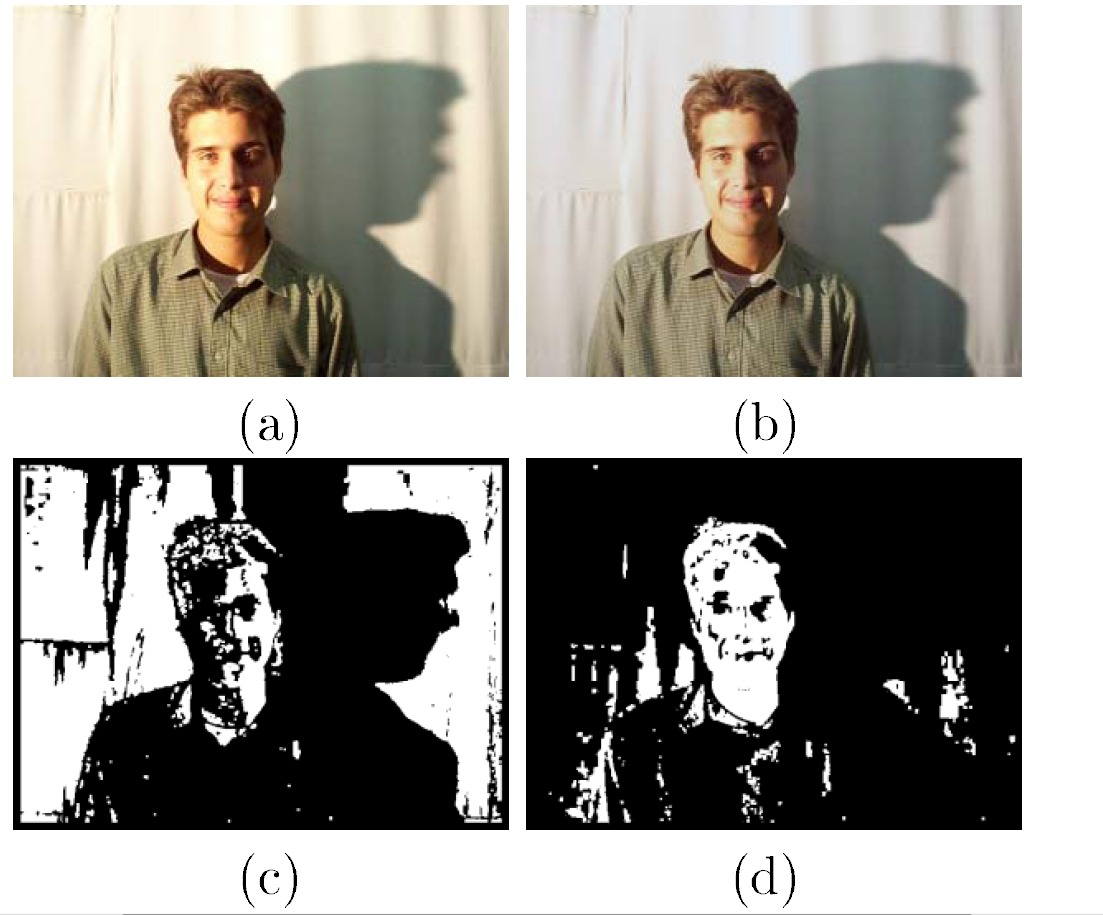
\includegraphics[width=\textwidth]{raw/skin_det.jpg}
\caption{Određivanje područja na slici koja pripadaju koži uz normalni i smanjeni utjecaj svijetlosti.}
\label{fig:skin_det}
\end{figure}

U drugom se dijelu postupka područja slike dobivena segmentacijom moraju klasificirati kao lica odnosno ne-lica zbog toga što se segmentacijom izdvajaju dijelovi slike koji odgovaraju koži što često uključuje i ostale dijelove tijela poput ruku. U radu \cite{Senior:2002:FDC:513073.513082} se tom problemu pristupa tako da se najprije odrede područja u kandidatima za lice koji odgovaraju očima i ustima te se lice prihvaća ako je ocjena pronađenih kandidata bolja od neke granične vrijednosti. 

\begin{figure}[!htb]
\centering
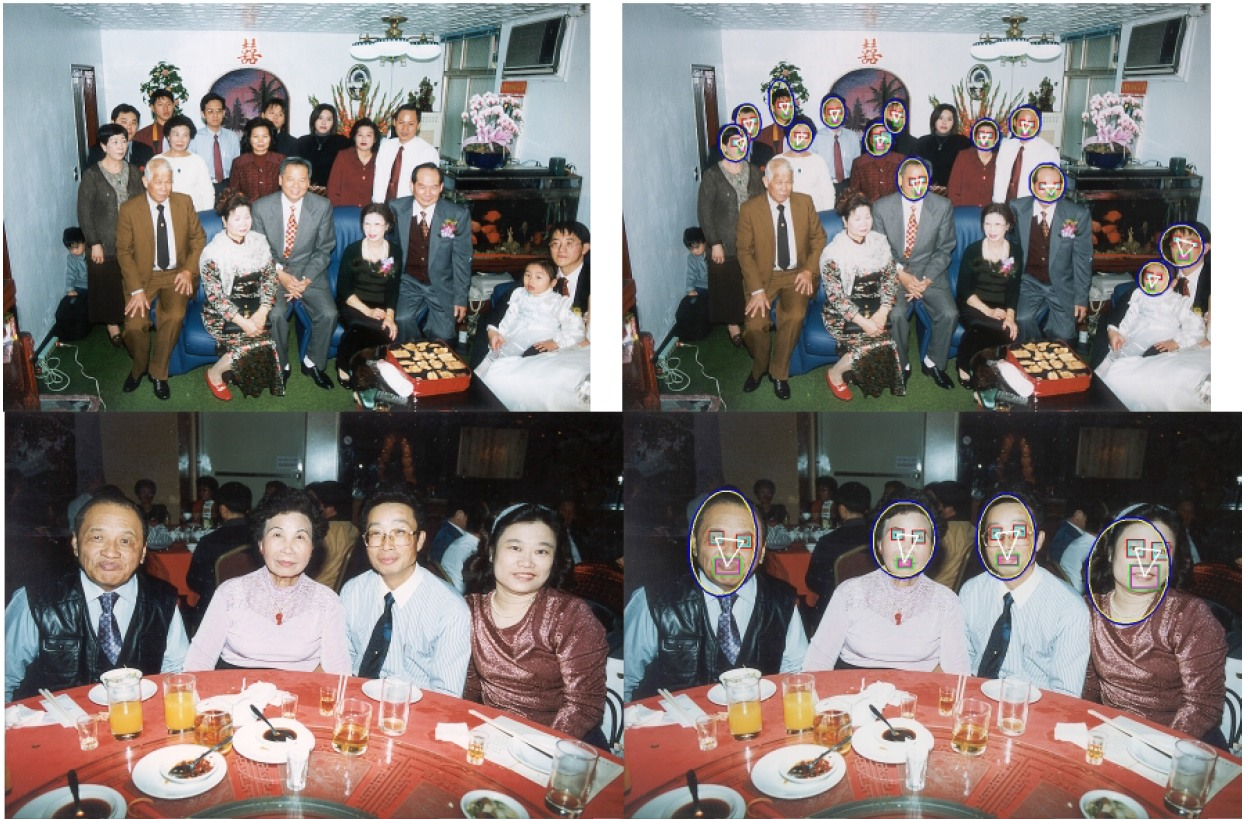
\includegraphics[width=\textwidth]{raw/detekcija_pr1.jpg}
\caption{Primjer detekcije lica u radu \cite{Senior:2002:FDC:513073.513082}.}
\label{fig:detekcija_pr1}
\end{figure}

Rad \cite{conf/isda/ChandrappaR12} ovom problemu pristupa na malo drugačiji način: na samom početku postoji skup lica koja čine skup za učenje, od tih se lica stvara slika prosječnog lica i za svakog kandidata lica se računa korelacija kandidata sa prosječnim licem. Ako je ta korelacija niska kandidat se odbacuje, inače ako je područje kandidata dovoljno veliko on se prihvaća kao područje lica. Test korelacije je sličan načinu na koji se maximal rejection classifier (MRC) koristi za detekciju lica opisanog u radu \cite{Elad00patterndetection}. Prihvaćanje kandidata na temelju veličine područja se obavlja koristeći prilagođavajuću granicu prihvaćanja kako bi se omogućilo prihvaćanje malih lica na slici, a istodobno odbacivalo manja područja za koje je prolazak testa korelacije moguć (dijelovi tijela poput ruku).

\begin{figure}[!htb]
\centering
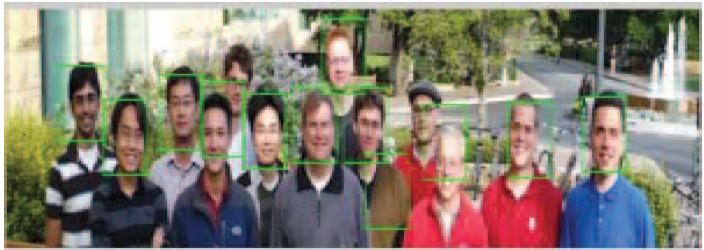
\includegraphics[width=\textwidth]{raw/detekcija_pr2.jpg}
\caption{Primjer detekcije lica u radu \cite{conf/isda/ChandrappaR12}.}
\label{fig:detekcija_pr2}
\end{figure}

\chapter{Predložena implementacija}

\chapter{Rezultati}

\chapter{Zaključak}
Zaključak.

\bibliography{literatura}
\bibliographystyle{fer}

\chapter{Sažetak}
Sažetak.

\end{document}
